

\documentclass[english]{article}
\usepackage[utf8]{inputenc}
\usepackage[margin=1in]{geometry}
\usepackage{graphicx,wrapfig,lipsum}
\usepackage{caption}
\usepackage{refstyle}
\usepackage{titlepic}
\usepackage{graphicx}
\usepackage{grffile}
\usepackage{babel}
\usepackage{parskip}
\usepackage{float}
\usepackage{subfigure}
\usepackage{graphicx}
\textwidth = 426pt
\oddsidemargin = 17pt


\title{COS 301 : User Manual\\
	for the SmartCard Application\\
	}
\date{\today}
\graphicspath{{Pictures/}}

\begin{document}
	\maketitle
	\begin{figure}[!t]
		
\includegraphics{up_logo.png}
	\end{figure}
	\begin{minipage}{0.4\textwidth}
		\begin{flushleft} \large
			\textbf{NAMES:}\\[0.4cm]
			Mufamadi {Khodani} \\
			Setoaba {Phuti} \\
			Dandashe {Kagiso Xolo} \\
		\end{flushleft}
	\end{minipage}
	\begin{minipage}{0.4\textwidth}
		\begin{flushright} \large
			\textbf{STUDENT NUMBER:} \\[0.4cm]
			u14197520 \\
			u13032616 \\
			u14245681 \\
		\end{flushright}
\end{minipage}

	
	\pagenumbering{gobble}
	\newpage

	\tableofcontents
	

	\pagenumbering{arabic}
	
\newpage
	\begin{figure}[!t]
		\centering
		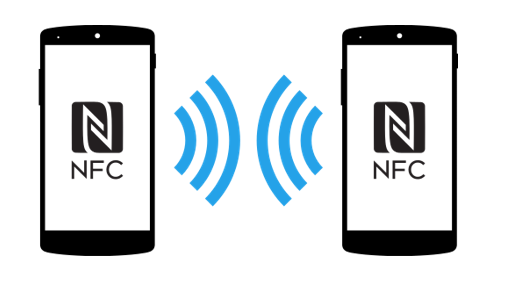
\includegraphics[scale=0.6]{NFC.png}
	\end{figure}

	\section{System Overview}
	The SmartCard system is a mobile-based application that is used to transfer business data from one device to another using either NFC or QR-Code scanner.The application should be free to download from either a mobile phone application store or similar services. 
	
	\section{System Configuration}
	The SmartCard system operates on mobile devices with Android operating system. It is compatible with
	Android 4,1 (jelly bean) API 16 and higher versions. The application requires connection to Internet in order to
	save data to database. A virtual business card will be generated for the user using the information the user signed up with and will then be transmitted with a single tap using the NFC too available on their smart device. Alternatively the smart device’s camera will be used to scan the QR code on another device. After
	installation on the device, SmartCard can be used immediately without any further configuration.
	\section{Installation}
	The most recent apk has been made available on our GIT repository link: https://github.com/XoloKDandashe/Alpha-Tech/tree/master/Smart\%20Business\%20Card\%20APK for installation on a device. 
	
	Download the apk from the website and install on your device. For specific instruction on how to install application on specific device refer to
	device’s manual.
	
	Alternatively the application should be available for download and install on google play store.
	

	\section {Using The System}
	\subsection{Getting started}
	Upon opening the system, the following screen will appear:
	
			\begin{figure}[H]
				\centering
			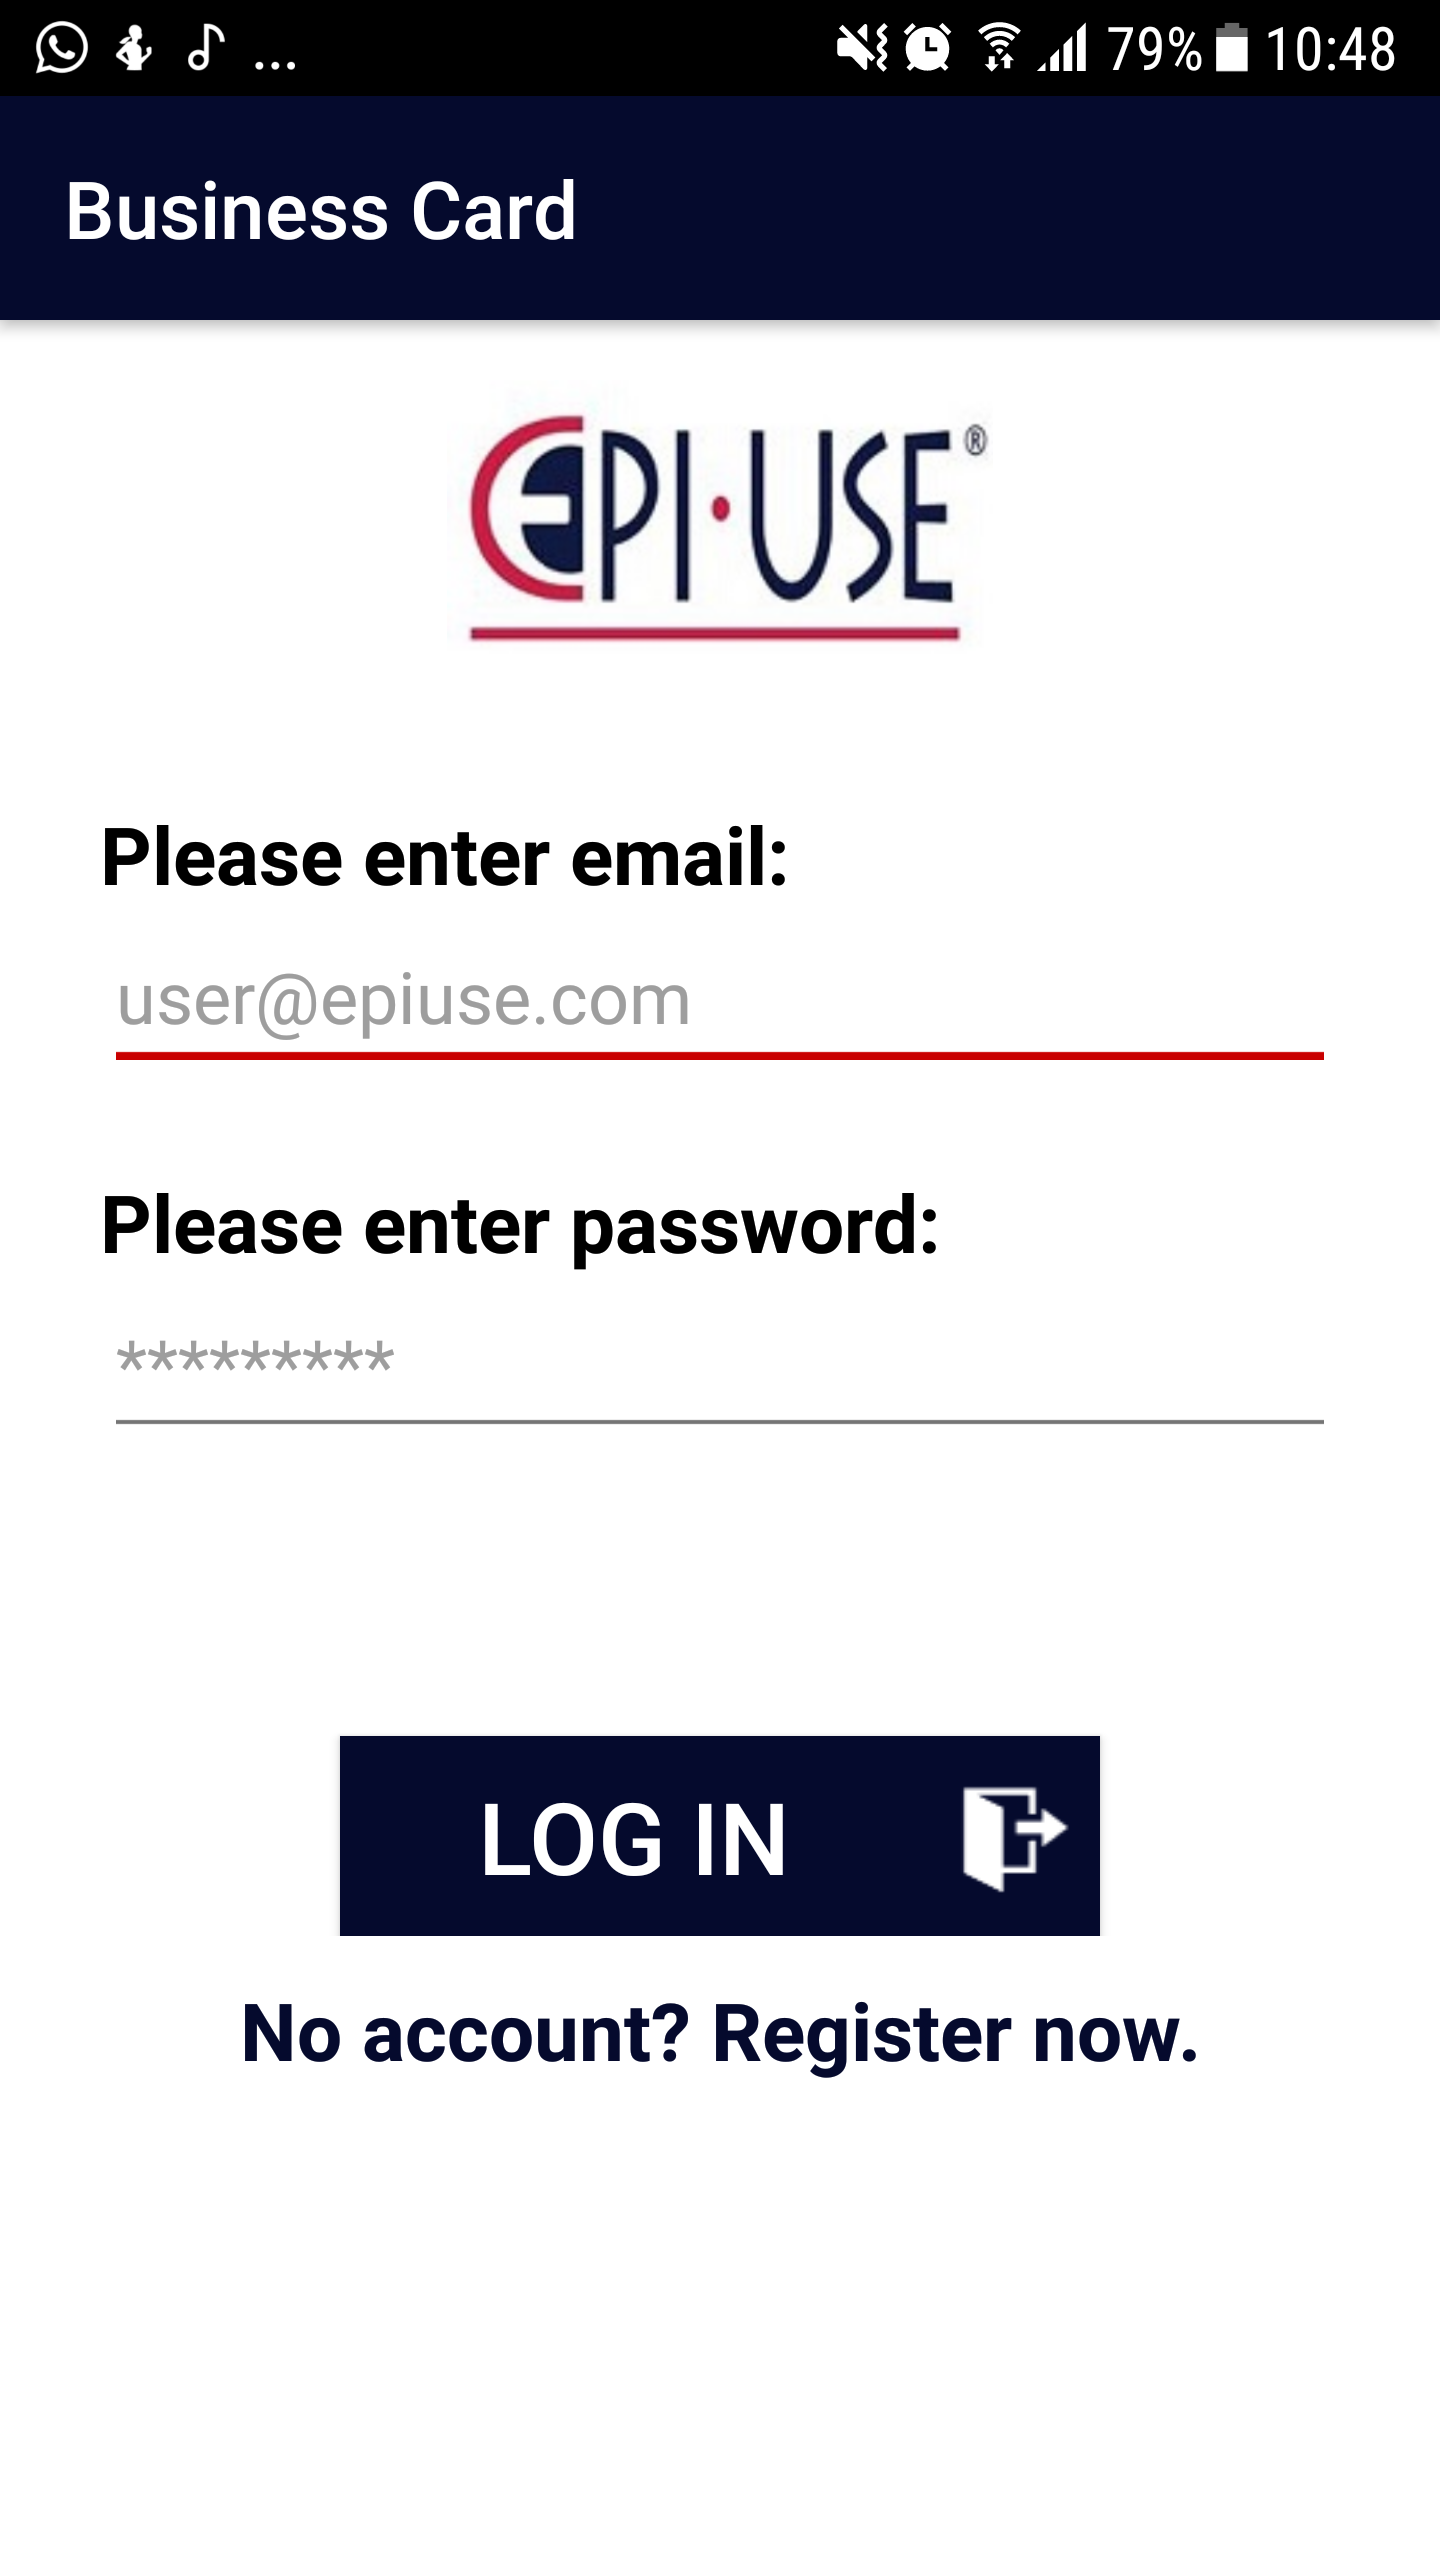
\includegraphics[scale=0.7]{Login.png}
				\caption{Log in page}
				\label{figure: 1}
			\end{figure}
			%\includegraphics[scale=0.7]{Login_def.png}

	\begin{itemize}
		\item How to login:
		\begin{itemize}
			\item Log in by using the email and password that were used when registering.
		\end{itemize}	
	\end{itemize}


	\begin{itemize}	
		\item How to Sign up manually:
		\begin{enumerate}
			\item Upon opening the application, select \textbf{\textit{Register now}} (Figure 1).
			\item Input your details on the provided form below.
			
			
			\begin{figure}[h!]
				\centering
				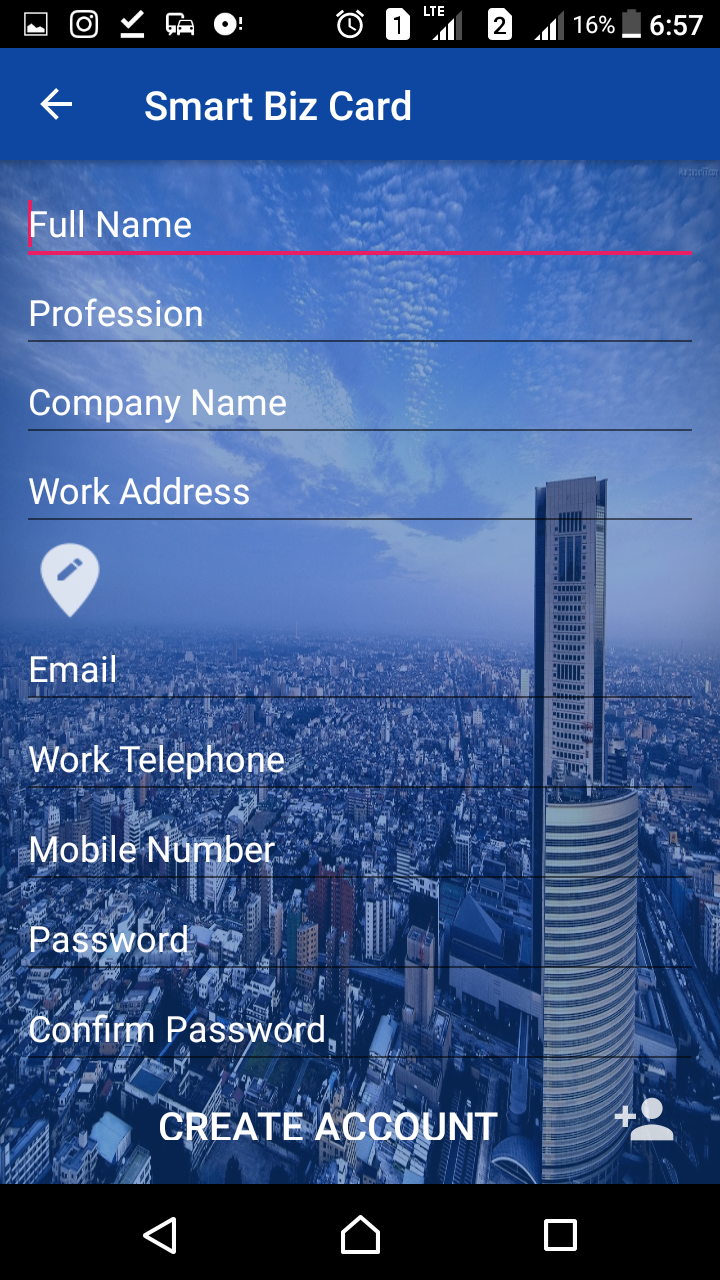
\includegraphics[scale=0.7]{Sign_up.png}
				\caption{Register form}
				\label{figure: 2}
			\end{figure}
		
			\item Select \textbf{CREATE ACCOUNT}.
				
			 
		\end{enumerate}
		\item How to Sign up via importing business card:
		\begin{enumerate}
			\item Upon opening the application, select \textbf{Import Business Card}.
			
			\begin{figure}[h!]
				\centering
				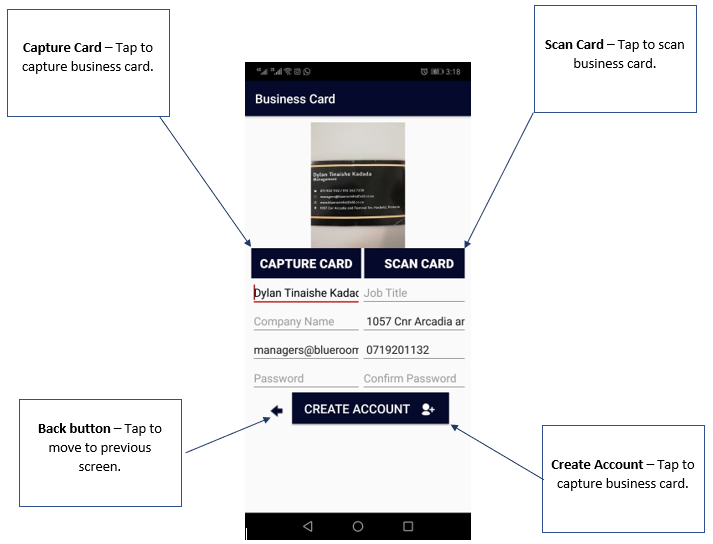
\includegraphics[scale=0.7]{scan_def.png}
				\caption{Import Card form}
				\label{figure: 3}
			\end{figure}
			%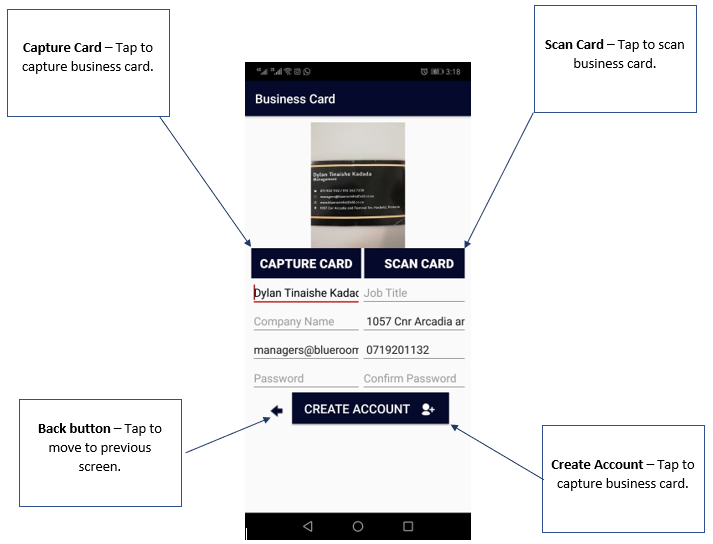
\includegraphics[scale=0.7]{scan_def.png}
			
			\item Select \textbf{CAPTURE CARD} to take a picture of the business card.
			\item After capturing, select \textbf{SCAN CARD} to enable the system to scan image and fill in the fields for you.
			\item If any fields were filled with incorrect information, you can rectify the mistakes by editing the fields manually.
			\item If any fields were not filled automatically, you can fill them in manually.
			\item Enter and confirm password then click \textbf{CREATE ACCOUNT}.
		\end{enumerate}
	\end{itemize}
	\begin{itemize}
		\item Main menu:
		\subitem After Registration or logging in, the following page will appear:
		
		\begin{figure}[H]
			\centering
			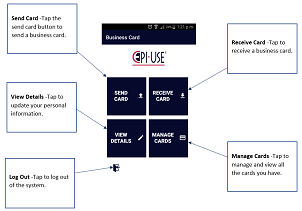
\includegraphics[scale=0.7]{Main_Menu.png}
			\caption{Main menu}
			\label{figure: 4}
		\end{figure}
	\end{itemize}



	\subsection{Sending business card}
		\begin{itemize}
		\item When the \textbf{SEND CARD} button is clicked, the following page appears:
		
		\begin{figure}[H]
			\centering
			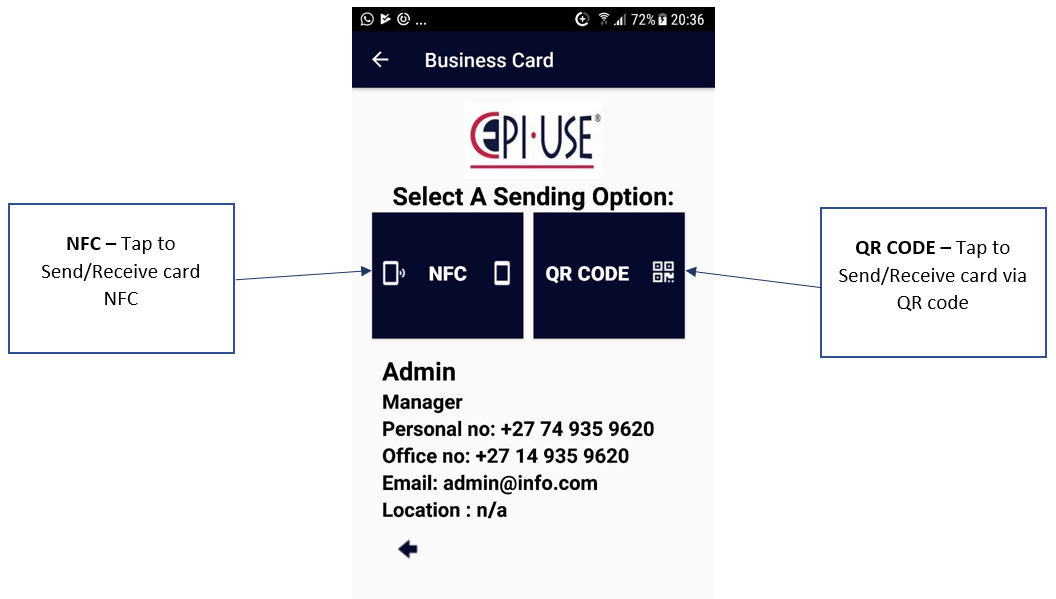
\includegraphics[scale=0.7]{swap_info.png}
			\caption{Swap business Card Menu}
			\label{figure: 5}
		\end{figure}
		
		\item Sending through NFC:
		\begin{enumerate}
			\item Select \textbf{NFC}
			\item Simultaneously tap the screen and touch the phone with another device.
		\end{enumerate}

		\item Sending through QR code:
		\begin{enumerate}
			\item Select \textbf{QR CODE}.
			\item Select \textbf{GENERATE CODE}.
			\item Allow another device to scan the code that was generated using their camera.
		\end{enumerate}
	\end{itemize}


\subsection{Receiving business card}
	\begin{itemize}
		\item Receiving through NFC
		\begin{enumerate}
			\item from a similar page to figure 5, select \textbf{NFC}
			\item Simultaneously tap the screen and touch the phone with another device.
		\end{enumerate}
		\item Receiving through scanning QR Code
		\begin{enumerate}
			\item from a similar page to figure 5, select \textbf{QR CODE}.  
			\item Select \textbf{SCAN CODE}.
			\item Scan the QR Code on another device to capture the data.
		\end{enumerate}
	\end{itemize}
\subsection{Manage Cards}
		\begin{figure}[H]
			\centering
			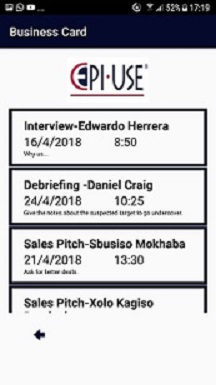
\includegraphics[scale=0.3]{Manage_Card.jpg}
			\caption{Manage cards}
			\label{figure: 6}
		\end{figure}
		\begin{itemize}
			\item When \textbf{MANAGE CARDS} option is clicked, the above view appears. 
		\end{itemize}
		
		\begin{figure}[H]
			\centering
			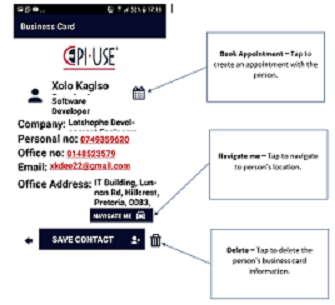
\includegraphics[scale=0.5]{person_info.png}
			\caption{View business card information}
			\label{figure: 7}
		\end{figure}
		\begin{itemize}
			\item When a card is clicked, the above view appears.
			\item When the dustbin icon is clicked, the user is asked to confirm if they want to delete that specific business card.
			\item Tap \textbf{NAVIGATE ME} to navigate to the persons company location.
			\item Tap the \textbf{Calendar icon} to create an appointment. 
		\end{itemize}
	\subsubsection{Create Appointment}
		\begin{enumerate}
			\item After the \textbf{calendar icon} is clicked in fig. 7, the following page appears:
			
			\item Enter the title, date, time and notes for the appointment.
			\item Tap on \textbf{SAVE APPOINTMENT} to create the appointment.
		\end{enumerate}
		
	\subsubsection{Navigate Me}
		\begin{enumerate}
			\item After clicking \textbf{NAVIGATE ME} in fig. 7, the following page appears:
			
			\item The companies location will appear on the screen.
		\end{enumerate}
	\section {Deployment diagram}
		\begin{itemize}
			\item The following components on the diagram are components that are already implemented:
			\begin{figure}[H]
				\centering
				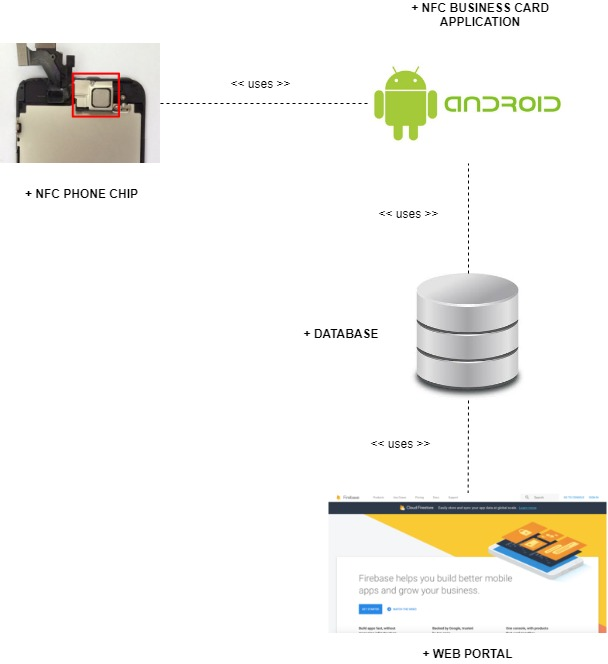
\includegraphics[scale=0.3]{Deployment.jpg}
				\caption{Deployment Diagram}
				\label{figure: 10}
			\end{figure}
		\end{itemize}
	\section {Troubleshooting}
		In case of failure to send or receive you will receive a pop up notification to let you know that the operation has failed and you will either have to try again or cancel the operation.
	
\end{document}
